%%==================================================
%% chapter04.tex for SJTU Master Thesis
%% Encoding: UTF-8
%%==================================================

\chapter{数据库驱动认知无线电网络中的位置推断攻击与保护}
\label{chap:fixed}

本章主要论述在数据库驱动认知无线电网络中固定用户所面临的位置隐私泄露以及相应的隐私保护方法。本章及后续部分所参考的依据主要为IETF发布的Internet草案和FCC公布的相关规定。

\section{系统模型}\label{sec:model}

在数据库驱动认知无线电网络中,我们假设数据库$DB$服务的区域$R$可以划分为$n \times n$个小区域,表示为$c_{ij}$,其中$i,j$分别是行索引和列索引。为方便描述,我们假定每个区域内的频谱可用信息相对稳定。网络中共有$C$个频道$ch_{1},...,ch_{k},...,ch_{C}$和$C$个主用户$PU_{1},...,PU_{i},...,PU_{C}$,即每个频道上有且只有一个主用户。可用频谱信息表示为$((ch_{1},P_{1},t_{1}),(ch_{2},P_{2},t_{2}),...,(ch_{k},P_{k},t_{k}))$。这里$ch_{i}$表示频道,$P_{i}$为$ch_{i}$上的允许发射功率,$t_{i}$为$ch_{i}$的预计可用时间。本文仅考虑可用频谱查询过程中的频道和功率信息,可用时间信息暂不列入考虑范围,因此可简化表示为$((ch_{1},P_{1}),(ch_{2},P_{2}),...,(ch_{k},P_{k}))$。可用频谱信息是数据库根据网络和地理环境进行计算的,主要考虑因素包括主用户的位置和发射参数、认知用户的发射参数、以及相关地理环境信息。认知用户允许发射功率$P_{i}$分为若干等级,由数据库根据最大传输功率(Maximum Transmission Power, MTP)函数进行计算得到。为方便起见,我们假设MTP函数只跟相对距离有关,即某个位置的认知用户在$ch_{i}$上所允许的最大发射功率$P_{i}$由该位置与$PU_{i}$所在位置的物理距离决定。公式\ref{eq:mtp}为MTP函数的一个示例。当距离小于$d_{0}$时,认知用户不允许发射以避免对主用户造成干扰;当距离超出范围$d_{n}$时,认知用户所允许的最大发射功率被定义为$P_{max}$,其具体值由FCC等机构规定,一般为100mW;当距离处于$d_{0}$和$d_{n}$之间时,认知用户允许以受限制的功率($<P_{max}$)工作。

\begin{equation}\label{eq:mtp}
P=\left\{
\begin{aligned}
&0  \quad when \ d(X)<d_{0} \\
&P_{1} \quad when \ d_{0} < d(X) \leq d_{1} \\
&... \\
&P_{max} \quad when \ d(X) > d_{n}
\end{aligned}
\right.
\end{equation}

基于IETF对数据库驱动认知无线电网络中可用频谱查询过程的规定,我们认为可用频谱查询的过程如下:

(1)请求:认知用户$SU_{i}$通过定位模块获取自身地理位置并向数据库发送请求消息,消息格式为$Que=(ID_{i},loc_{i})$。$ID_{i}$是$SU_{i}$的设备标识符及唯一身份标识,$loc_{i}$是$SU_{i}$的地理位置。我们假定认知用户可以同时查询其附近多个地理位置的可用频谱信息。

(2)响应:数据库在收到查询消息并提取地理位置信息后,计算该位置可用频谱信息并向认知用户发送响应消息,消息格式为$Res=(c_{ij},ch_{i},P_{i})$。

(3)通知:尽管在IETF制定的草案中,这个步骤是可选的,但是数据库作为网络中的服务提供者和管理者,需要根据认知用户的接入情况计算可用频谱信息,因此我们假定认知用户需要上报使用的频道信息,消息格式为$Not=(ID_{i},ch_{i},P_{i})$。


\section{针对静止用户的位置推断攻击}\label{sec:attack-fixed}

根据上述可用频谱查询过程,$DB$可以直接获得$SU$的地理位置信息。文献\cite{gao2013location}提出了一种基于私有信息提取的盲化查询机制,使得认知用户的地理位置信息在查询过程中对数据库是不可见的。事实上,即便在不直接获取认知用户位置的前提下,我们仍然可以根据可用频谱查询过程中的通信内容与用户位置的相关性对用户位置进行推测。因此,本文提出的攻击方法假设数据库无法直接获得认知用户的地理位置。本节工作主要考虑网络中主用户和认知用户都静止的情况。

如上所述,在可用频谱查询过程中,$DB$向$SU$提供某些地理位置上的可用频谱信息,包括可用的频道$ch_{i}$和该频道允许的最大发射功率$P_{i}$。由于$ch_{i}$所允许的发射功率$P_{i}$主要由认知用户与该频道主用户$PU_{i}$之间的距离所决定,因此认知用户可以根据$P_{i}$对它与$PU_{i}$之间的距离进行估算从而经过若干轮查询后能够逐渐确定$PU_{i}$的位置。认知用户在确定使用的频道$ch_{i}$后,需要向$DB$上报$ch_{i}$以及$P_{i}$。类似地,$DB$可以对认知用户与$PU_{i}$之间的相对距离进行估算,进而在经过若干轮查询后逐渐确定认知用户的位置。我们发现在频谱查询过程中,无论响应消息还是通知消息,都可以表示为一个可用频谱信息单元$(ch_{i},P_{i})$,而每个单元都含有一定的相对距离信息,从而可以根据MTP函数将$(ch_{i},P_{i})$转换为一个区域覆盖范围,进而我们基于网络中可能出现的两种隐私泄露情况提出如下相应的两种位置推断攻击。

\subsection{基于受限功率的位置推断攻击}
$DB$向认知用户提供的可用频谱信息可以简化为若干个可用频谱单元:$((ch_{1},P_{1}),...,(ch_{i},P_{i}),...,(ch_{C},P_{C})$。最大传输功率$P_{i}$被分为若干离散的功率等级,从而能够提高网络的服务效率。在理想的情况下,我们可以假设每个功率等级的覆盖范围为圆形区域或圆环型区域。如图\ref{fig:limited}所示,若认知用户$SU_{i}$收到关于$ch_{i}$的可用频谱信息单元$(ch_{i},P_{i})$,则它可以认为自己与主用户$PU_{i}$之间的距离大致在$d_{1} \sim d_{2}$之间,即$PU_{i}$有较大的概率处于左侧图中阴影环形区域内。同理,若$SU_{i}$上报的使用频道的最大发射功率为$P_{i}$,则$DB$可以认定$SU_{i}$有较高的概率处于右图中阴影区域内。

\begin{figure}[!htp]\label{fig:limited}
  \centering
  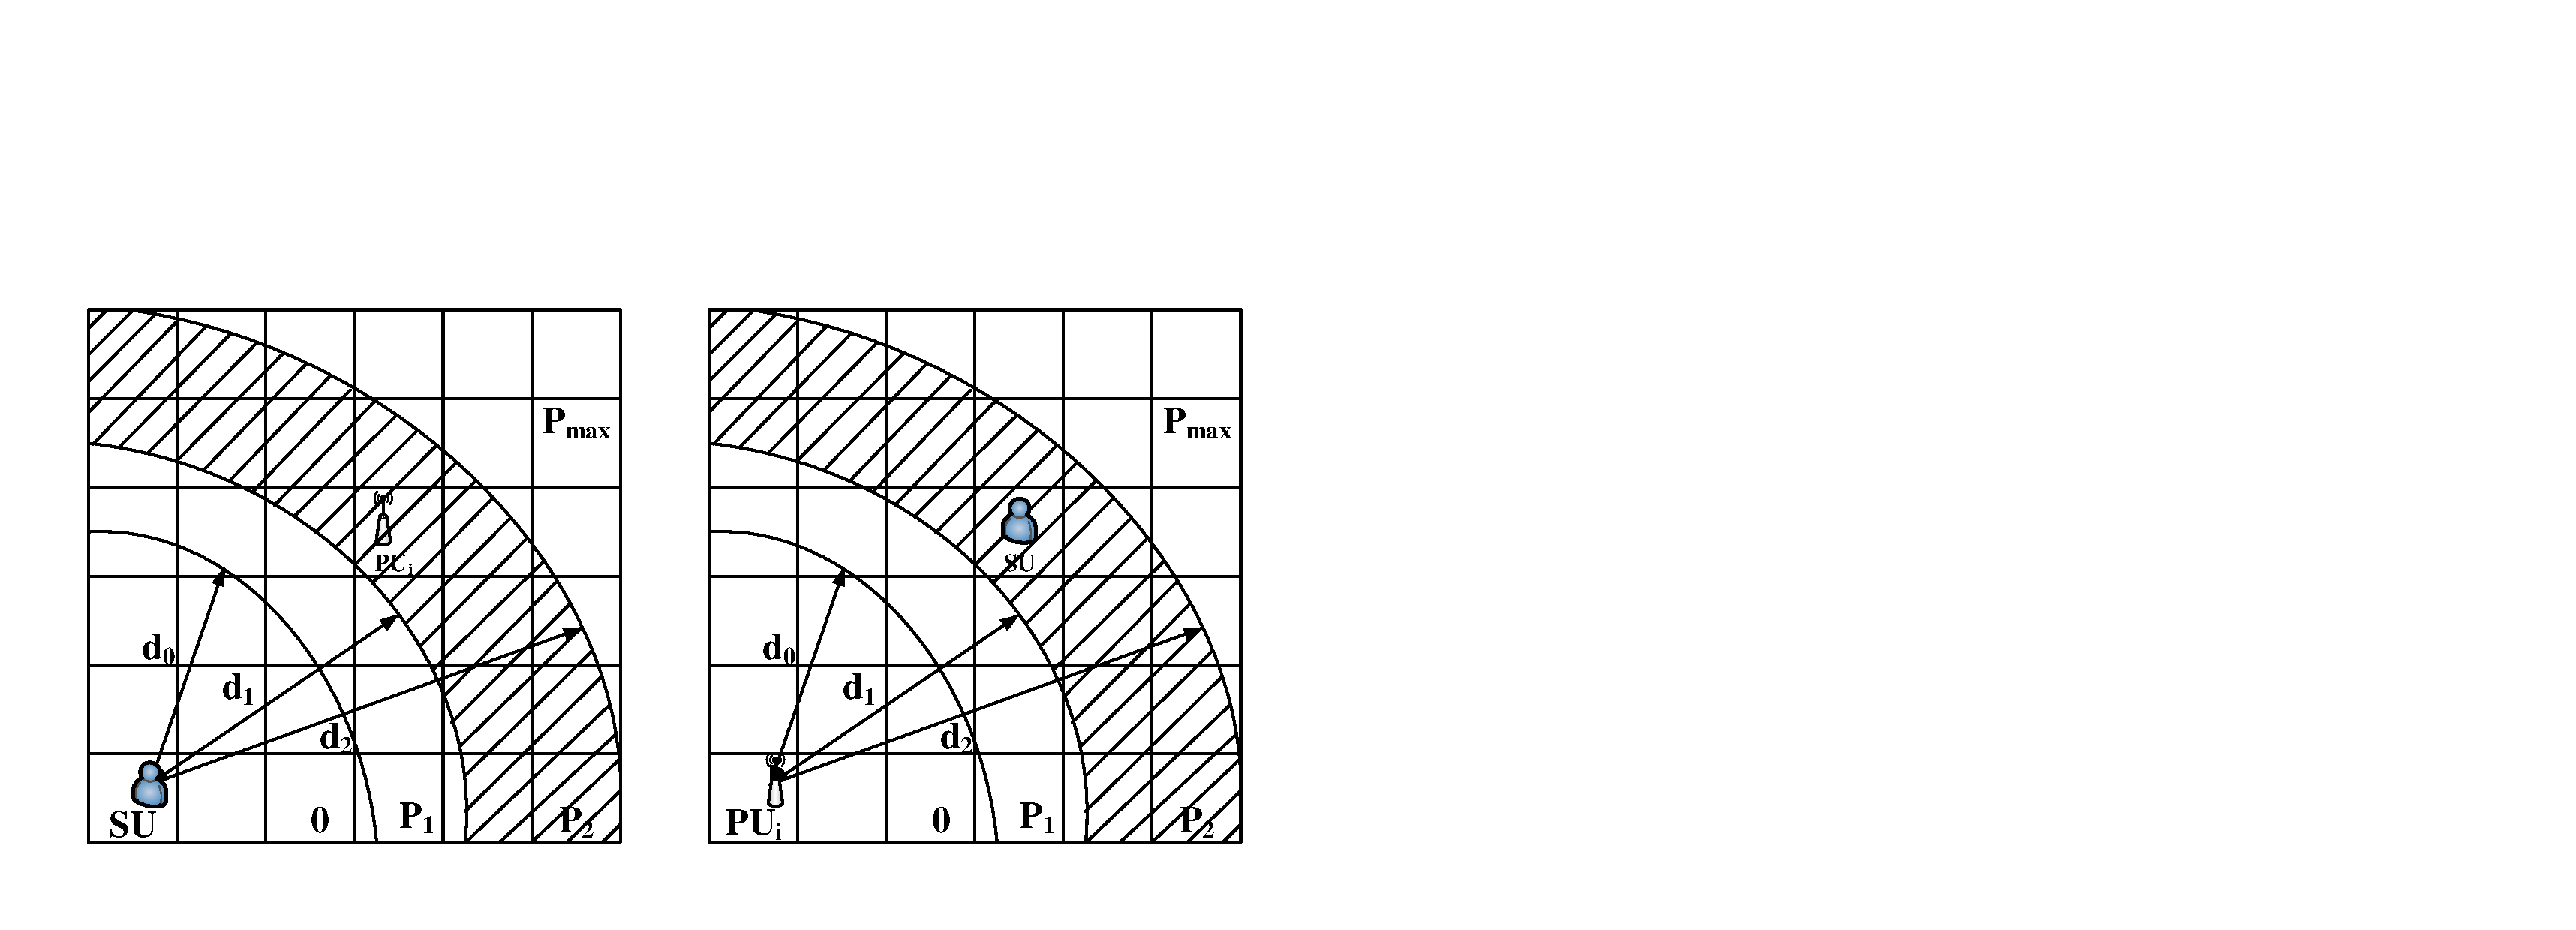
\includegraphics[width=0.8\textwidth]{figures/chap4/limited}\bicaption[fig:attack:limited]{基于受限功率的位置推断攻击示意图}{基于受限功率的位置推断攻击示意图}{Fig}{Illustration of Attack Based on Limited Power}
\end{figure}

若$SU_{i}$持续选择功率受限的频道,那么随着时间的推移,攻击者可以将每一次的覆盖范围进行取交集操作从而实现对静止的$SU_{i}$的比较精确的位置推断。

\subsection{基于频道切换的位置推断攻击}

为确保认知用户在使用频谱过程中不会对主用户产生任何干扰,当主用户在线时,认知用户不允许在主用户的保护范围内以相同的频道发射功率。主用户的保护区域一般是一个以主用户为圆心的圆形区域,假设保护区域半径为$d_{0}$。当主用户$PU_{i}$在线时,这个区域内不允许任何认知用户在$ch_{i}$工作。因此可能出现的一种情况是,$PU_{i}$不在线,某个认知用户$SU_{i}$处于主用户$PU_{i}$的保护范围内且正在使用$ch_{i}$,一旦$PU_{i}$上线,则$DB$会通知$SU_{i}$立即腾出$ch_{i}$。基于这个切换事件,$SU_{i}$立即得知,$PU_{i}$有很大概率处于以$SU_{i}$所在位置为圆心,以$d_{0}$为半径的圆形区域内。同理,若$DB$计算出某个$SU_{i}$不允许在$ch_{i}$上发射,则$DB$可以认为$SU_{i}$有较大概率处于$PU_{i}$的保护范围内。基于频道切换的位置推断攻击如图\ref{fig:switch}所示。

\begin{figure}[!htp]\label{fig:switch}
  \centering
  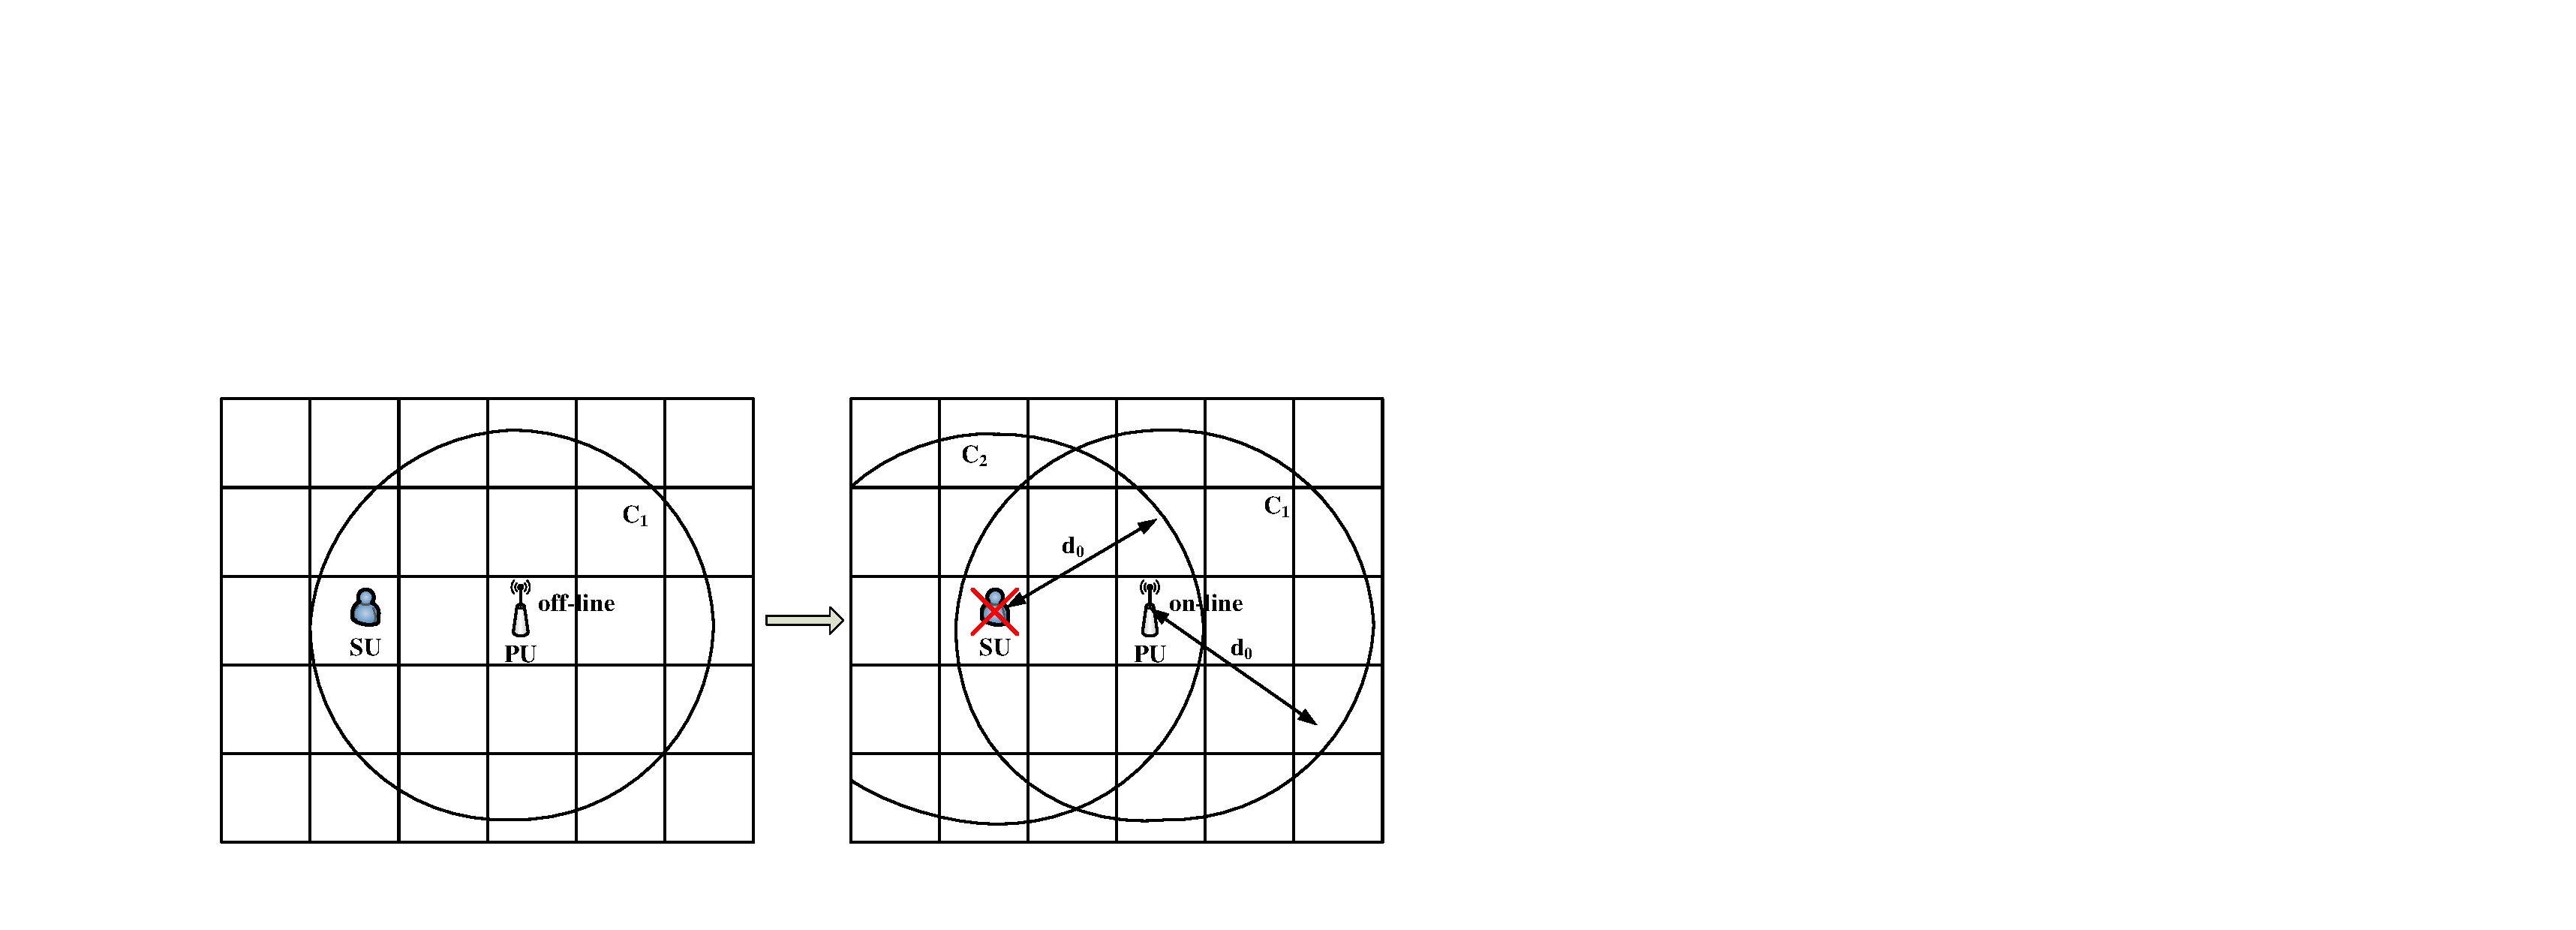
\includegraphics[width=0.8\textwidth]{figures/chap4/switch}\bicaption[fig:switch]{基于频道切换的位置推断攻击示意图}{基于频道切换的位置推断攻击示意图}{Fig}{Illustration of Attack Based on Channel Switch}
\end{figure}

由于主用户的保护范围为圆形区域,覆盖范围相比其他情况要小,因此频道切换事件会更加严重地泄露认知用户和主用户的位置隐私。

\subsection{统一的位置推断攻击算法}\label{alg-attack}

根据如上分析,在数据库驱动认知无线电网络中,认知用户和数据库在位置推断攻击的层面上是对立的。一方面认知用户可以根据数据库提供的可用频谱信息危害网络中主用户的位置隐私;另一方面数据库可以根据提交的频道信息危害认知用户的位置隐私。因此,我们认为在可用频谱查询过程中主用户和认知用户的隐私同时存在被对方攻击的风险。根据可用频谱查询过程中认知用户和数据库之间传输的可用频谱信息单元$(ch_{i},P_{i})$,我们提出了一种一般化的攻击方案。算法\ref{alg:fixed}是该攻击方法的伪代码描述。

\begin{lstlisting}[language={C}, caption={统一的位置推断攻击算法}]
输入:攻击者的位置$loc$,频谱单元序列$((ch_{1},P_{1}),...,(ch_{i},P_{i}),...,(ch_{C},P_{C})$;攻击者先验知识$R'$。
输出:目标的可能位置集$L$
初始化:$L=\phi$;  $\delta$;  $n \times n$概率矩阵$PR$,$pr_{ij} \in PR$
for $0 \leq i \leq n$ and $0 \leq j \leq n$
    if $c_{ij} \in R'$
        $pr_{ij}=\frac{1}{2}$
    else
        $pr_{ij}=0$
for each ($ch_{i},P_{i}$)
    if 功率受限或频道切换事件发生
        M=Cov($ch_{i},P_{i}$) 
            for each $c_{ij} \in Cov(ch_{i},P_{i})$
                $pr_{ij}=\frac{pr_{ij}}{1-\frac{1}{|M|}(1-pr_{ij})}$ 
                if $pr_{ij} \geq \delta$
    $L = L \cup c_{ij}$
    return $L$
Cov($ch_{i},P_{i}$):
    $d_{min},d_{max}$ = $P_{i}$对应距离范围的边界值
    X = $\phi$
    for $c_{ij} \in R'$
        if $d_{min} \leq distance(c_{ij},loc) \leq d_{max}$
            $X = X \cup c_{ij}$
    return X
\end{lstlisting}\label{alg:fixed}

在算法\ref{alg:fixed}中,攻击者可能具有对目标的先验知识,即目标的可能位置分布,这可以缩小对目标位置的推测范围。$M$代表频谱信息单元$(ch_{i},P_{i})$对应的覆盖范围,$|M|$是范围内包含的小区域数量。我们根据公式\ref{eq:bayes}所述的贝叶斯规则\cite{bahrak2013ex},在每一轮迭代中将可能作为候选的区域对应的概率值逐渐增加,直到超过预先设定的阈值$\delta$,则认定该区域可能是攻击目标所处的位置。我们将在本章最后对攻击效果进行验证。
\begin{equation}\label{eq:bayes}
pr_{ij}=\frac{pr_{ij}}{1-\frac{1}{|M|}(1-pr_{ij})}
\end{equation}

\section{针对位置推断攻击的解决方案}

为解决数据库驱动认知无线电网络中静止用户的隐私泄露问题,我们必须同时考虑两个方面的问题:服务质量和隐私保护。在数据库驱动认知无线电网络环境下,服务质量即为频谱效益。对认知用户来讲,它是网络服务的使用者,主要关注自身所能够获得的频谱质量;对数据库来讲,它是整个网络的服务提供者,需要为全局尽量提供较好的频谱质量。一般来讲,无论对于服务提供者还是服务使用者,服务质量和隐私保护效率都是一对矛盾的双方。例如在传统的LBS中,用户如果想获得更好更准确的周边信息服务,那就必然要向服务提供者提交更加精确的位置,因而也会导致位置隐私泄露更加严重。任何隐私保护的方案一定是以牺牲某方面的服务性能为代价的。在本节,我们提出一个频谱查询过程中的隐私保护框架,使得认知用户和数据库可以根据自身需求,在满足一定服务质量的前提下,最好地保护自身隐私。为方便描述,我们必须首先对服务质量和隐私给出一个量化的定义。

\subsection{频谱效益和隐私的度量}

\subsubsection{频谱效益的度量}

对于频谱效益,我们可以直观地采用无线信道容量作为其度量标准。信道容量是由通信链路上的信号与干扰噪声强度比来决定的(Signal to Interference and Noise Ratio, SINR),认知用户获得的通信链路的SINR可由公式\ref{eq:SINR}计算\cite{capacity}。

\begin{equation}\label{eq:SINR}
SINR  = \frac{P_{sec}/L_{sec}(r_{cell})}{N_{0}W_{0}+I_{P2S}+I_{S2S}}
\end{equation}

在公式\ref{eq:SINR}中,$P_{sec}$为认知用户的发射功率,$L_{sec}(r_{cell})$为小区域中认知用户发射接收链路的损耗。$N_{0}$为认知用户接收机的噪声功率谱密度,$W_{0}$是认知用户的信道带宽,$I_{P2S}$是主用户对认知用户的干扰,$I_{S2S}$是认知用户之间的干扰。

在小区域$c$内的频道$ch_{i}$上获得的平均信道容量可以由公式\ref{eq:capacity}表示\cite{capacity}。
\begin{equation}\label{eq:capacity}
Cap_{c}^{i}  = W_{0} \int_{c} \frac{log_{2}(1+SINR(l))}{c}dl
\end{equation}

为简化实际模型的表示,我们假设信道容量在小区域$c$范围内相对稳定,因此可将认知用户在$ch_{i}$上获得的信道容量重写为:
\begin{equation}\label{eq:capacity-revised}
Cap_{c}^{i}  = W_{0} log_{2}(1+SINR^{i})
\end{equation}

对于网络中的认知用户,他们只关心所使用频道的容量而与数据库提供的其他可选频道无关,因此认知用户的频谱效益可以表示为公式\ref{eq:util-su}。
\begin{equation}\label{eq:util-su}
Util_{SU}=\frac{1}{|CH|}\sum\limits_{ch_{i} \in CH} Cap_{c}^{i}
\end{equation}
式中$CH$为认知用户使用过的频道列表,$|CH|$为集合元素个数,上式的意义为认知用户历史上使用过的频谱服务总量。


对于数据库来说,他关心为每个用户所提供的总的服务能力,因此提供的可选择频道越多,频道的容量越大,则服务质量越好,于是我们使用公式\ref{eq:util-db}来表示数据库针对某个认知用户的频谱效益:
\begin{equation}\label{eq:util-db}
Util_{DB}=\frac{1}{|CH_{A}|} \sum\limits_{ch_{i} \in CH_{A}} Cap_{c}^{i}
\end{equation}

$CH_{A}$是数据库为认知用户提供的可用频道的集合,$|CH_{A}|$为集合元素个数。公式\ref{eq:util-db}的意义是数据库为某个认知用户提供的平均信道容量。

\subsubsection{隐私的度量}

对位置隐私进行度量的常用方式是采用位置的不确定性。假设可能的位置集为$L=(l_{1},l_{2},...,l_{n})$,在这些位置上的概率分布为$(p_{1},p_{2},...,p_{n}),\sum\limits_{i=1}^{n} p_{i} = 1$。根据熵公式,位置不确定性可表示为公式\ref{eq:uncertainty}:
\begin{equation}\label{eq:uncertainty}
UnC=-\sum\limits_{i=1}^{n}p_{i}log p_{i}
\end{equation}

使用不确定性作为隐私度量方式的问题是,它无法准确地描述攻击者对位置的估计误差。此外,基于我们提出的攻击算法,攻击目标处于可能位置集合$L$中所有位置的概率是相等的,都是$1/|L|$,其中$|L|$是集合$L$中元素个数。因此,我们可采用平均误差距离作为隐私的度量方式。我们将\ref{alg-attack}中的攻击算法表示为条件概率密度函数$A(loc'|\cdot)$,$\cdot$为算法中的输入信息,$loc'$为攻击者推断出的位置。那么隐私可以表示为公式\ref{eq:privacy}。

\begin{equation}\label{eq:privacy}
Priv=\sum\limits_{loc' \in L} A(loc'|\cdot)d(loc,loc')
\end{equation}

其中函数$d()$是两个位置之间的欧氏距离,$loc$为攻击目标的真实地址,$loc'$为攻击者推断的地址。


\subsection{隐私保护的频谱查询方案}\label{subsec:privacy-preserving}

为减少可用频谱查询过程中的位置隐私泄露,我们提出一种改进的频谱查询方案如下:
\subsubsection{基于$k$-anonymity的请求}
认知用户同时查询包含$K_{Q} \times K_{Q}$个小区域的正方形区域$B$内的可用频谱信息。若考虑节省通信开销的问题,可以从$B$中随机挑选若干位置进行查询。认知用户可以将周边区域的可用频谱信息作为频道选择的参考。图\ref{fig:cloaking}为基于$k$-anonymity的请求示意图。

\begin{figure}[!htp]\label{fig:cloaking}
  \centering
  \includegraphics[width=0.8\textwidth]{figures/chap4/cloaking}\bicaption[fig:cloaking]{基于$k$-anonymity的可用频谱请求示意图}{基于$k$-anonymity的可用频谱请求示意图}{Fig}{Available Spectrum Query Based on $k$-anonymity}
\end{figure}

\subsubsection{基于$k$-anonymity的响应}
为弱化攻击者对主用户位置的推理攻击,我们采用文献\cite{bahrak2014protecting}中提出的基于$k$-anonymity的隐私保护方案,将网络中的主用户进行分组的办法来保护主用户的位置隐私。具体方法是将距离最近的主用户划分为若干个组,每一组有至少$K_{R}$个用户。我们认为每一个用户组是一个虚拟的主用户,其保护区域覆盖了内部所有主用户的保护区域。这样,数据库根据虚拟的主用户信息来计算可用频谱信息,在牺牲一些可用频谱资源的前提下,能够在一定程度上模糊主用户的真实位置,如图\ref{fig:anonymity}所示。

\begin{figure}[!htp]\label{fig:anonymity}
  \centering
  \includegraphics[width=0.8\textwidth]{figures/chap4/anonymity}\bicaption[fig:anonymity]{基于$k$-anonymity的可用频谱响应示意图}{基于$k$-anonymity的可用频谱响应示意图}{Fig}{Illustration of Available Spectrum Response Based on $k$-anonymity}
\end{figure}
在对主用户进行分组时,我们首先尽量选择最近的$K_{R}$个主用户分为一组,然后我们需要找到能够覆盖这$K_{R}$个位置的最小覆盖圆。假设最小覆盖圆的圆心为$X$,半径为$R_{X}$,则我们可以通过解决如下问题来找到$X$和$R_{X}$。

\begin{equation}
\min_{X} \max_{loc_{i}} {d(loc_{i},X)}
\end{equation}
其中,$loc_{i}$为主用户的地址,函数$d()$为两个点之间的欧氏距离。
然后我们可以将MTP函数修改为:
\begin{equation}\label{equation:mtp-altered}
P(loc)=\left\{
\begin{aligned}
&0  \quad when \ d(loc,X)<R_{X}+ d_{0} \\
&P_{1} \quad when \ R_{X}+d_{0} < d(loc,X) \leq R_{X}+d_{1} \\
&... \\
&P_{max} \quad when \ d(loc,X) > R_{X}+d_{n}
\end{aligned}
\right.
\end{equation}

这种基于$k$-anonymity的方法显然会增加主用户的位置隐私,因为它明显扩大了主用户的保护范围。同时,也必然会带来明显的频谱效益下降。此外,参数$K_{R}$的值对数据库的频谱效益和能够获得的隐私保护程度影响非常大,我们在后面讨论$K_{R}$的选择。

\subsubsection{改进的频道选择}

根据\ref{sec:attack-fixed}节分析的隐私泄露方式,若认知用户随机地选择满足要求的频道,则会遇到更多的功率受限和频道切换的情况,从而导致严重的隐私泄露。因此,在基于$k$-anonymity的可用频谱请求和响应的基础上,我们提出提出如下频谱选择方案。
(1)认知用户在所有查询的区域上都收到可用频谱信息单元$(ch_{i},P_{max})$,那么该认知用户有可能离主用户$PU_{i}$很远,也有可能意味着$PU_{i}$不在线。若是第二种情况而且认知用户恰好处于$PU_{i}$的保护范围内,那么很可能发生频道切换事件。因此,建议不使用这类频谱资源。
(2)认知用户在其所处的区域收到可用频谱信息单元$(ch_{i},P_{max})$,然而在其查询的其他区域关于$ch_{i}$的最大可用功率不全为$P_{max}$,那么说明$PU_{i}$一定在线,而且认知用户的位置距离主用户很远。这类可用频道既能允许较高的发射功率,又能较少的泄露位置隐私,因此较为推荐使用。
(3)认知用户在其所处的区域没有收到允许最大功率发射的可用频谱单元,那么他应该挑选允许发射功率最大的频道来使用,因为允许发射功率越大的频道对应的覆盖范围越大,而且信道质量越好。

\subsubsection{参数决定}
在上面提出的隐私保护的可用频谱查询框架中,为了在满足一定的频谱效益的前提下实现隐私保护的最大化,我们需要确定最合适的参数和选项。
对于数据库来讲,他应该力图在保证提供一定质量服务的前提下尽可能保护主用户隐私。因此根据前面的定义,我们可将数据库的频谱效益写为:

\begin{equation}
Util_{DB}=\frac{1}{K_{R}^{2}}\sum\limits_{c \in B} \sum\limits_{ch_{k} \in CH_{A}} Cap_{k}
\end{equation}

数据库的隐私保护程度可写为:

\begin{equation}
Pri_{PU}(loc,S(K_{Q},K_{R}))=\sum\limits_{loc' \in L} A(loc'|SAI(K_{Q},K_{R}))d(loc,loc')
\end{equation}

式中,$SAI(K_{Q},K_{R})$表示参数为$K_{Q},K_{R}$的情况下$DB$提供的可用频谱信息。若我们设定$\sigma_{DB}$为$DB$可忍受的最小频谱效益,则可以通过解决如下问题来得到最优的参数$K_{R}$。

\begin{equation}
\max_{K_{R}} Priv_{PU}(loc_{PU},SAI(K_{Q},K_{R})) 
\end{equation}

\begin{equation}
s.t. \quad Util_{DB} \geq \sigma_{DB}
\end{equation}

对于认知用户来讲,由于他们不知道网络中主用户的位置,所以无法自己计算隐私泄露程度,只能通过上面提出的方法优先选择合适的频道。但是在网络设计者的角度,我们可以给出类似的隐私定义并在具有网络全局知识的前提下,通过解决如下问题来计算能最大化认知用户隐私的最优频道:

\begin{equation}
\max_{ch_{i}} Priv_{SU}(loc_{SU},CH \cup ch_{i}) 
\end{equation}

\begin{equation}
s.t. \quad Util_{SU} \geq \sigma_{SU}
\end{equation}

式中$\sigma_{SU}$是认知用户所能容忍的最低的频谱效益。

\subsection{位置推断攻击与隐私保护的实验验证}
我们对文中提出的攻击方法和隐私保护方法的有效性进行了实验验证。从目前网络上公布的广播电视频段信号强度数据库来看,网络中的主用户即电视发射台一般集中部署,因此网络中大部分主用户几乎处于同一位置。然而未来的数据库驱动认知无线电网络一定不会局限于此类部署方式。因此,本文采用随机模拟的场景进行实验。

我们考虑数据库服务于一个$40km \times 40km$的区域,该区域划分为$400 \times 400$个$100m \times 100m$的正方形小区域。区域内有50个主用户、50个频道和随机分布的若干认知用户。假设最大传输功率量化为4个等级:0、1、2、3,其中等级0为不允许发射,等级3为$P_{max}$,其对应的覆盖范围如公式\ref{eq:coverage}所示。在数据库服务区域内,主用户随机切换在线/离线状态但不会太频繁。在不影响整体结果的条件下,度量频谱效益和隐私时,我们忽略了主用户对认知用户的干扰以及认知用户之间的干扰,直接采用功率等级来衡量信道容量。
\begin{equation}\label{eq:coverage}
P=\left\{
\begin{aligned}
&0 \quad when \ d < 8km \\
&1 \quad when \ 8km \leq d < 14km \\
&2 \quad when \ 14km \leq d < 25km \\
&3 \quad when \ d \geq 25km
\end{aligned}
\right.
\end{equation}
图\ref{fig:exp1-su}展示了对认知用户的攻击效果。可以看出,由于认知用户随机选择接入的频道,那么随着时间的增加,各种受限功率和频道切换事件发生的次数增加,于是导致其位置隐私逐渐泄露。一段时间之后,各种可能导致位置隐私泄露的事件都发生过,则认知用户可以最终被定位在一个较小的区域范围内,平均定位精度约25个小区域,范围大致相当于一个$500m \times 500m$的正方形区域。

\begin{figure}[!htp]
  \centering
  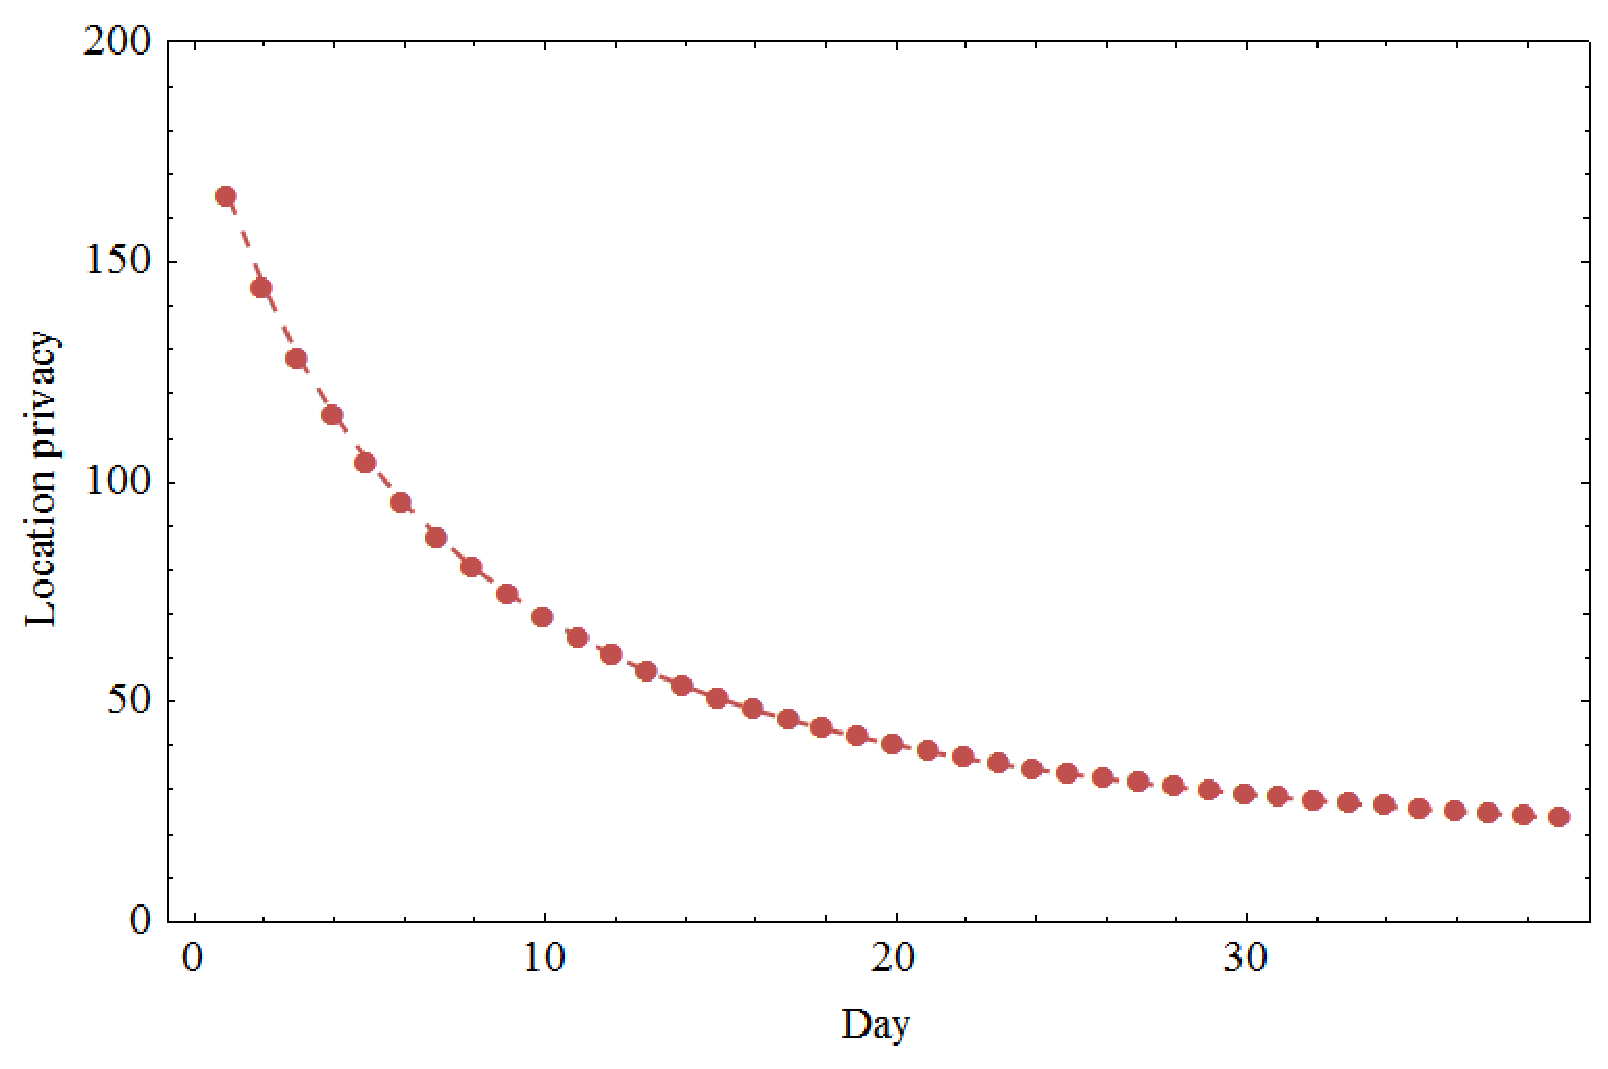
\includegraphics[width=0.55\textwidth]{chap4/exp1-su}
  \bicaption[fig:exp1-su]{认知用户的位置隐私泄露}{认知用户的位置隐私泄露}{Fig}{Location Privacy Leaking of Secondary Users}
\end{figure}

图\ref{fig:exp2-pu}展示了对主用户实施位置推断攻击的效果。可以看出,随着时间的增加,主用户的位置隐私泄露地更加明显,最终可能被攻击者锁定在5个小区域内,这个很高的定位精度源于数据库提供的丰富的而且细粒度的可用频谱信息。

\begin{figure}[!htp]
  \centering
  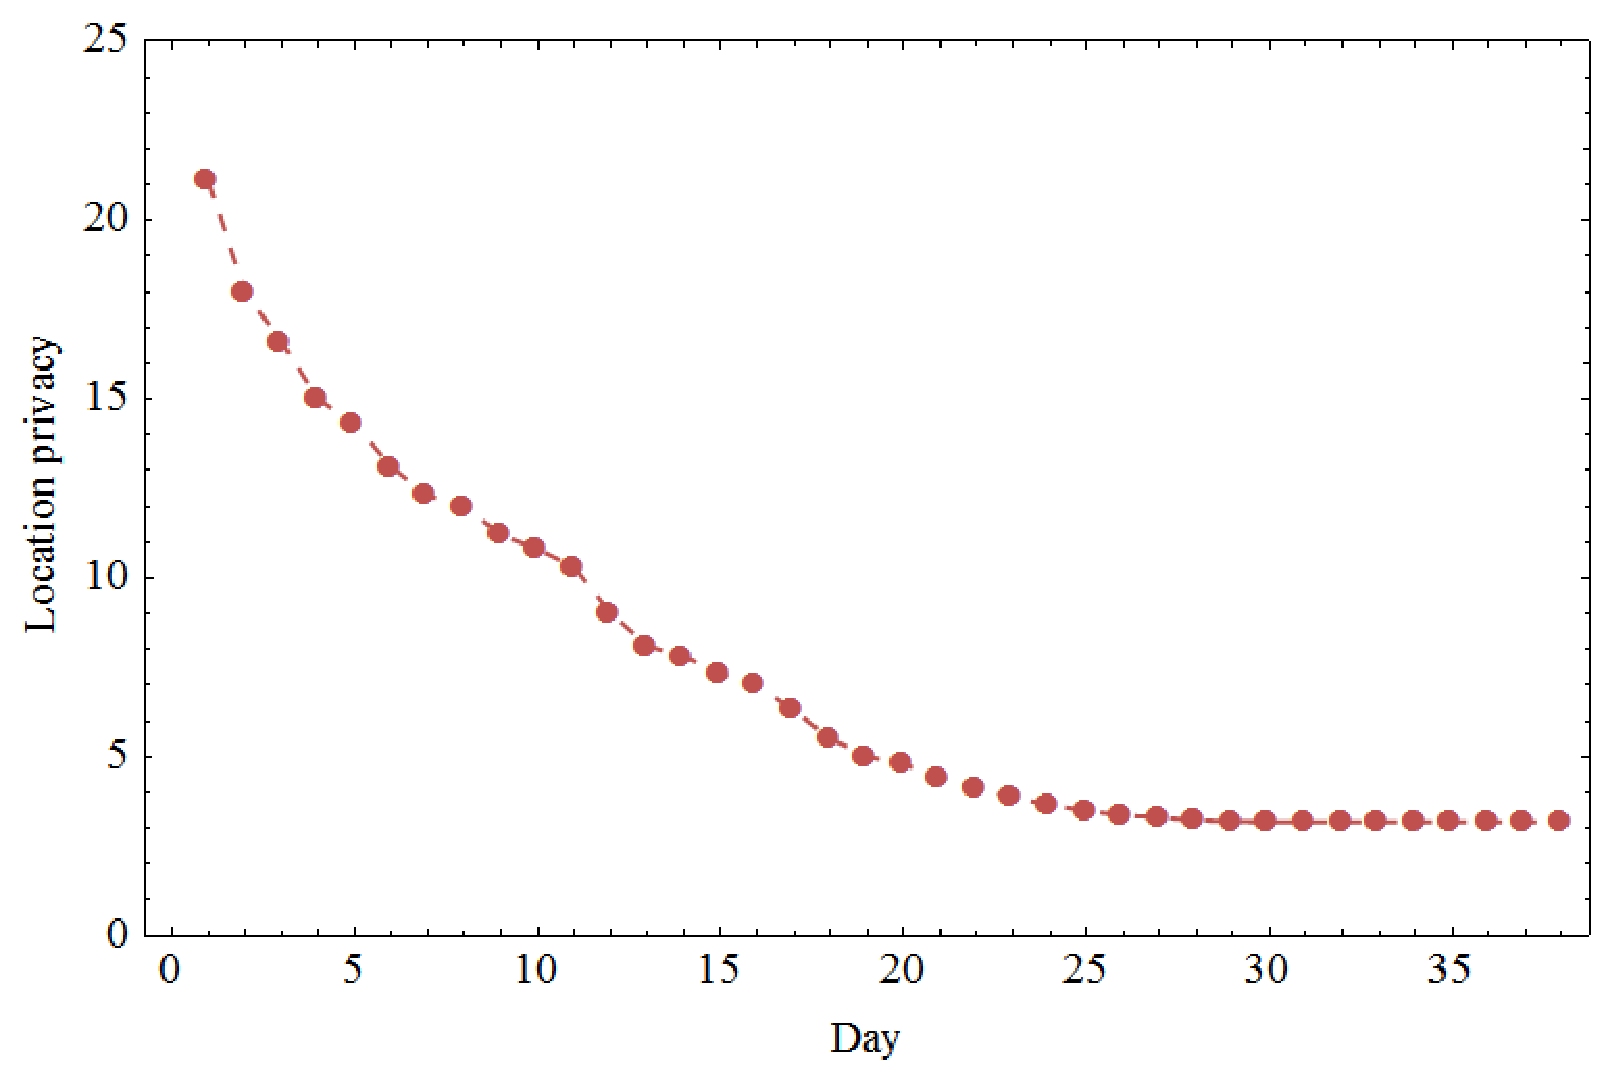
\includegraphics[width=0.55\textwidth]{chap4/exp2-pu}
  \bicaption[fig:exp2-pu]{主用户的位置隐私泄露}{主用户的位置隐私泄露}{Fig}{Location Privacy Leaking of Primary Users}
\end{figure}

我们对提出的隐私保护的可用频谱查询方案进行了实验验证,并与之前的查询方案进行了对比。在采用隐私保护的可用频谱查询前后,我们分别随机采样了若干认知用户来分析频谱效益和隐私保护。在图\ref{fig:exp3-su}中,标注random的曲线簇意味着随机选取接入频道,标注为optimal的曲线簇意味在文中提出的隐私保护框架下能够实现的最优结果。容易得知,在没有采用隐私保护措施时,认知用户即使在牺牲很多频谱效益的情况下也无法获得满意的隐私保护程度。若采用隐私保护的频谱选择策略,则认知用户理论上能够实现的隐私保护程度将大大提高,但无法避免由此带来的频谱效益的下降。

\begin{figure}[!htp]
  \centering
  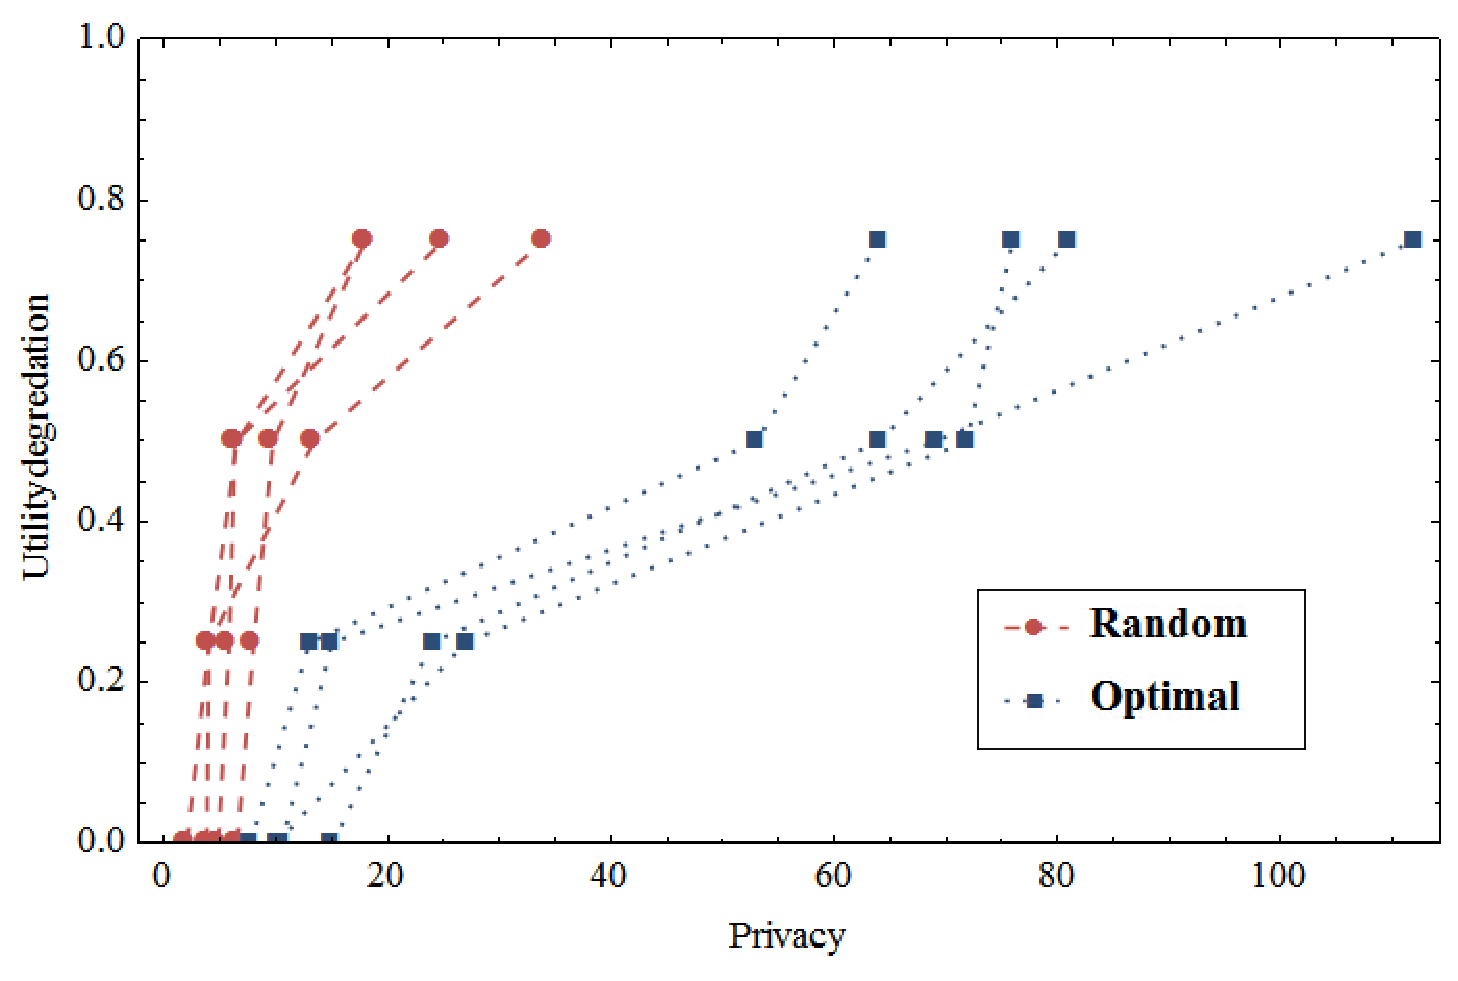
\includegraphics[width=0.6\textwidth]{chap4/exp3-su}
  \bicaption[fig:exp3-su]{认知用户的频谱效益与隐私}{认知用户频谱效益与隐私}{Fig}{Spectrum Utility and Location Privacy of Secondary Users}
\end{figure}

我们也分析了主用户采用隐私保护手段后的效果。在图\ref{fig:exp4-pu}中,标注为random的曲线意为数据库随机选择$K_{R}$的值来计算可用频谱,标注为optimal的曲线意为数据库在最优值的情况下能够达到的频谱效益和隐私保护的折中。我们可以看出,基于$k$-anonymity的频谱响应可以显著提高隐私保护程度,而且通过合理地选择$K_{R}$,我们还可以大大减少频谱效益的下降。

\begin{figure}[!htp]
  \centering
  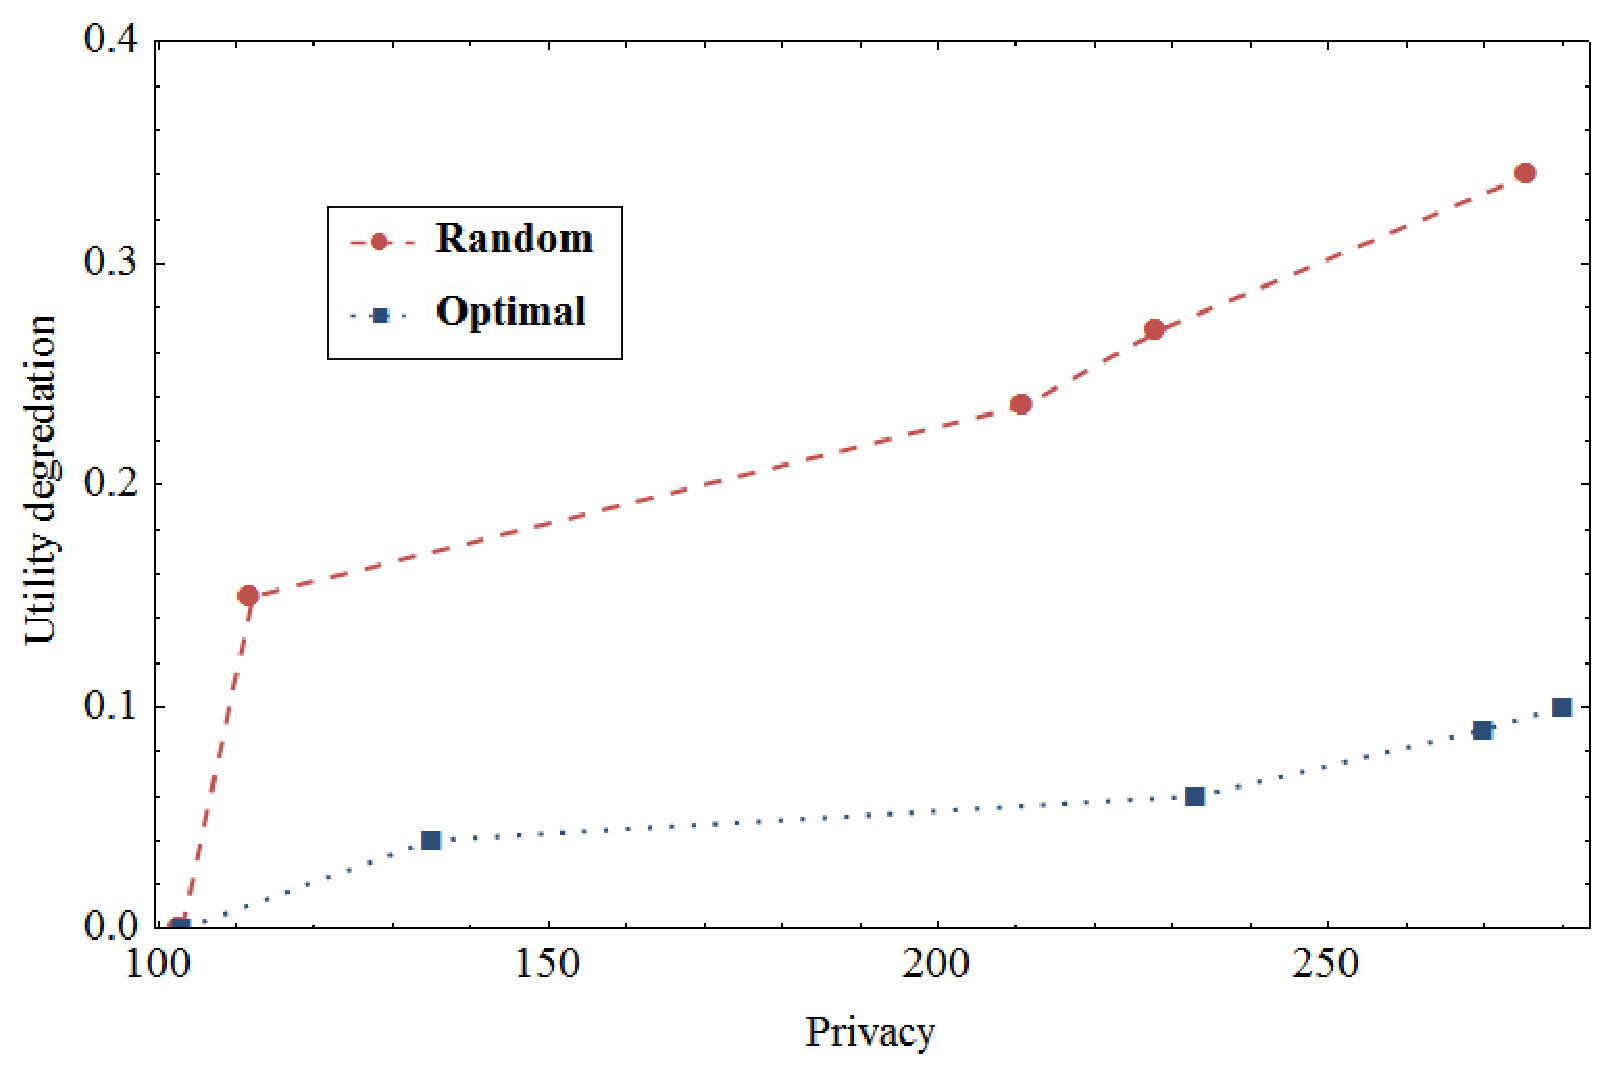
\includegraphics[width=0.6\textwidth]{chap4/exp4-pu}
  \bicaption[fig:exp4-pu]{数据库的频谱效益与隐私}{数据库的频谱效益与隐私}{Fig}{Spectrum Utility and Location Privacy of Primary Users}
\end{figure}

我们还可以预测,若认知用户选择了较大的$K_{Q}$值,则数据库会提供更多位置的频谱可用信息从而为认知用户选择使用频道提供详细的知识,但是更丰富的频谱可用信息也意味着主用户的隐私泄露更多,因此数据库反而可能会增大$K_{R}$的值来减少主用户隐私泄露,那么也相应导致数据库频谱效率的降低。由于认知用户在不清楚网络中主用户具体位置的前提下无法在本地确定隐私泄露的情况,而且动态调整$K_{Q}$和$K_{R}$的复杂度较高,所以本文没有对$K_{Q}$的取值对隐私保护的影响进行研究。

